\part{Hybrid Ground Control Systems}

This year's hybrid control system is a completely new project for avionics with no prior system to inform its design.
The current working prototype is an Arduino based control system which has been difficult to maintain and use. The
system was designed using breadboard electronics and it is very difficult to organize the jumper wires or perform
repairs on the system. It also does not have the ability to detect connection interruptions, the user interface does
not update at the speed desired for monitoring the system and it has a tendency to crash spuriously. This prototype
system has sufficed for preliminary testing of the hybrid in cold flows, but must be updated for static fire testing
and launch.

\section{Network Infrastructure}

The hybrid control system will be network based to make use of the robust protocols which already exist for
communication over a network. The primary components of the network control system are Ubiquity Litebeam M5 dishes for
long range wireless networking, pictured in Figure \ref{fig:ubiquity-dish}. This avoids the need for Ethernet cabling
exceeding 2,000 feet, which is inconvenient to set up.

\begin{figure}[H]
    \center
    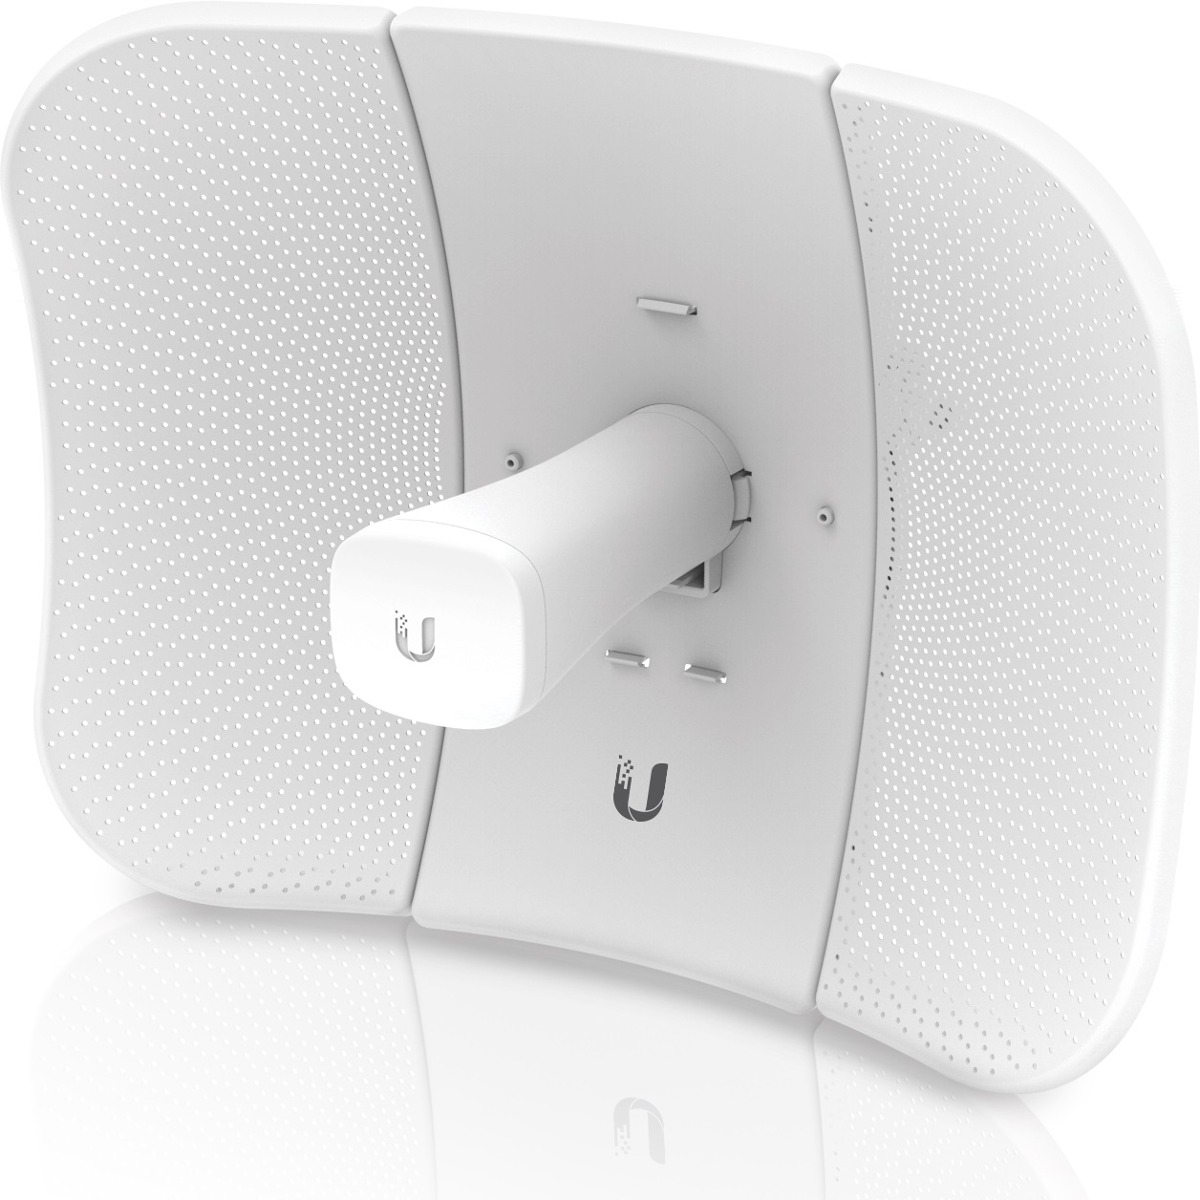
\includegraphics[width=2in]{assets/images/ubiquity-dish.jpg}
    \caption{Ubiquity Litebeam M5 wireless dish \cite{ubiquity-dish}}
    \label{fig:ubiquity-dish}
\end{figure}

\subsection{Topology}

\subsection{Control System Nodes}

The communication within the hybrid control system network is centred around three distinct node types:

\begin{itemize}
    \item Telemetry clients
    \item Control client
    \item Pad control server
\end{itemize}

All of these nodes communicate with each other according to the hybrid control system communication specification,
which can be found in Appendix \ref{apx:comm-spec-repos}.

\subsubsection{Telemetry Clients}

Telemetry clients are simply consumers of the telemetry data produced by the pad control server. There can be a
theoretically infinite number of telemetry clients on the network at once, and they can all consume the same data being
sent by the pad control server. This is possible through the use of \gls{udp} multicast.

Telemetry clients are free to do whatever they would like with the telemetry data they receive. This could be simply
logging it to a file, performing a statistical analysis or using it to update status LEDs/hardware on a physical
device. The hybrid control UI is an example of a telemetry client which displays the data it receives visually.

\subsubsection{Control Client}

A control client is able to issue commands to the pad server. Only one control client is permitted to be connected to
the pad server at once. This is done to prevent the receipt of conflicting commands from two controllers, eliminating a
large suite of possible race conditions.

The commands sent from a control client are either arming commands or commands for actuating (turning on or off)
actuators. Control clients are simple in that they only send these commands to the pad server and wait for a response
indicating success or failure of the command. An example interaction can be seen in Figure \ref{fig:cntrl-pad-seq}.

\begin{figure}[H]
    \center
    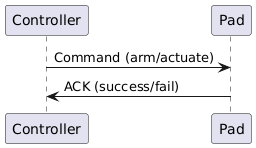
\includegraphics[width=2in]{assets/diagrams/control_client_and_pad_sequence.png}
    \caption{Control client to pad server communication sequence diagram}
    \label{fig:cntrl-pad-seq}
\end{figure}

Control clients \textbf{do not} maintain any state about the actuators they control, they only blindly issue commands
and receive indication of success or failure. In this way, all state is maintained on the pad server which preserves a
single source of truth in the system. This makes it impossible for the control client to get out of sync with the real
system state.

Commands sent from a control client to the pad server are done using \gls{tcp}. \Gls{tcp} was chosen because it is a
reliable, connection-based protocol, which enables the either end of the connection to detect when the other has
disconnected. This can be used to determine failures in the control system.

\subsubsection{Pad Server}

The pad server is the most complicated of the nodes. The pad server produces all the telemetry data from the system
sensors, which it sends over \gls{udp} multicast. This design allows a theoretically infinite number of telemetry
clients to consume telemetry data, while the server only has to perform a single "send" operation.

The pad server simultaneously handles incoming commands from the control client, to which it responds with a success or
failure acknowledgement. The pad server is responsible for maintaining internal state about the actuators and current
arming level, which it uses to decide whether the command is currently possible. For example, a command to ignite the
igniter is not allowed until the main valve for the oxidizer has been opened, and that itself depends on a sequence of
prior conditions. There is a progression of arming escalation which must be adhered to.

\begin{figure}[H]
    \center
    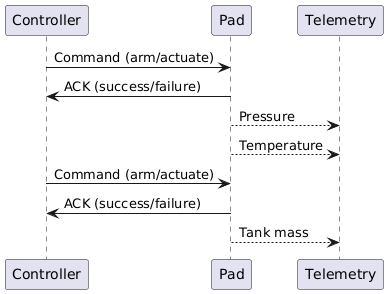
\includegraphics[width=2in]{assets/diagrams/all_nodes_seq.png}
    \caption{Example communications between all the network nodes}
\end{figure}

Responding to commands from the control client is prioritized above telemetry. At the top priority is the emergency
abort sequence for dumping the oxidizer in the tank when pressure spikes above nominal levels are detected, or when
network connection has been lost for a predefined time duration.

\subsubsection{Combination Nodes}

Combination nodes are those nodes which implement both the control client and telemetry client nodes on one system.
This may be useful for a control box with a heads up display for telemetry readings, which the operator may need to use
to inform command decisions. These systems can use telemetry data to inform sending commands, etc.\ but should still
never store any state about the system. All state information can be queried from the pad server.

\section{Arming Logic}

The control logic that the pad server uses to govern which actuation and arming commands are valid at any given time
are based on the arming state \gls{fsm} in Figure \ref{fig:arming-fsm}.

\begin{figure}[H]
    \center
    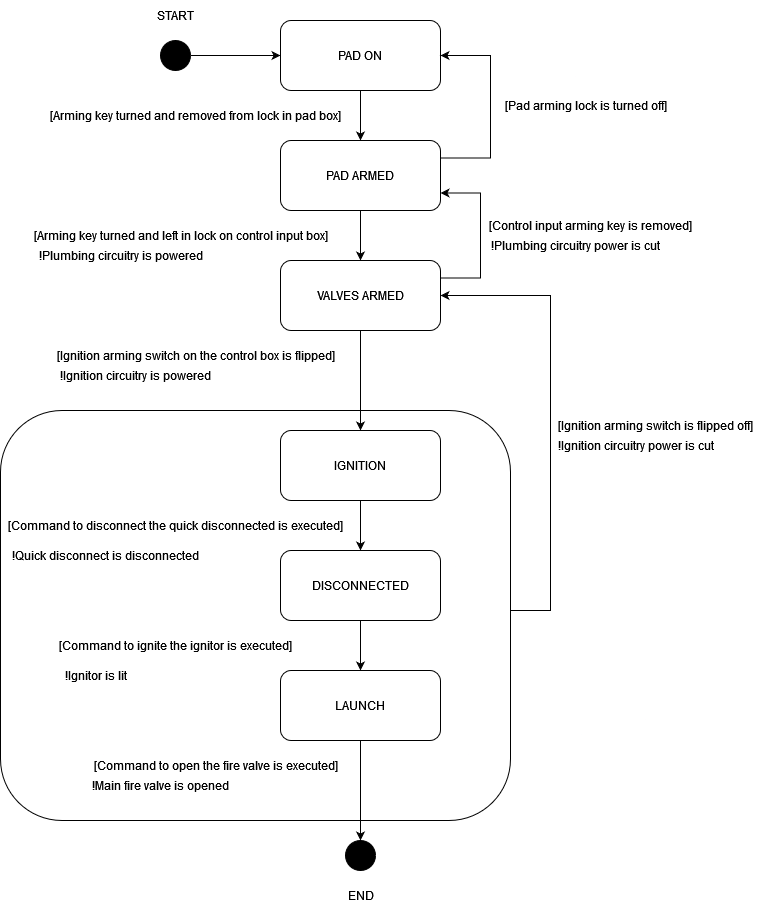
\includegraphics[width=4in]{assets/diagrams/Hybrid_Control_FSM.png}
    \caption{Arming state \gls{fsm} for the pad server}
    \label{fig:arming-fsm}
\end{figure}

This \gls{fsm} defines transitions based on command inputs from the control client. Transitions are sometimes triggered
by arming commands, which specifically request that the \gls{fsm} jump to a given state. Such commands are a virtual
stand-in for physical arming circuitry. For instance, it is not possible to enter the \textit{VALVES ARMED} state to
control the valves until the control box is armed (see the condition on the transition from \textit{PAD ARMED}). This
arming is performed using a physical arming key, which is the same key shared to arm the pad box. Such a mechanism
ensures that the pad team has physically returned back to the remote control box with the arming key in order to arm
the system for valve control, which means they are a safe distance from the active plumbing. Since the electrical
signal of the key being turned in the control box cannot be wirelessly sent to the pad, a network command is instead
used to indicate that the arming has taken place. This is the purpose of arming commands.

Other times, transitions are based on a specific sequence of actuations. For example, transitioning from the
\textit{IGNITION} state to the \textit{DISCONNECTED} state requires that the quick disconnect be actuated. This ensures
that the ground system plumbing to the hybrid motor is no longer connected to the rocket before it is possible for the
operator to ignite the motor for liftoff. Otherwise, the plumbing would be taken for quite a ride.

Each arming state progression from top to bottom in Figure \ref{fig:arming-fsm} comes with elevated privileges.
Privileges are described in the hybrid communication protocol specification in Appendix \ref{apx:comm-spec-repos}. For
instance, solenoid valves for tank filling and venting can be controlled in the \textit{VALVES ARMED} state and higher.
\cite{hybrid-comms} Opening the main fire valve (which allows the oxidizer to flow onto the lit igniter) is only
permitted in the \textit{LAUNCH} state.
